\begin{figure}
\centering
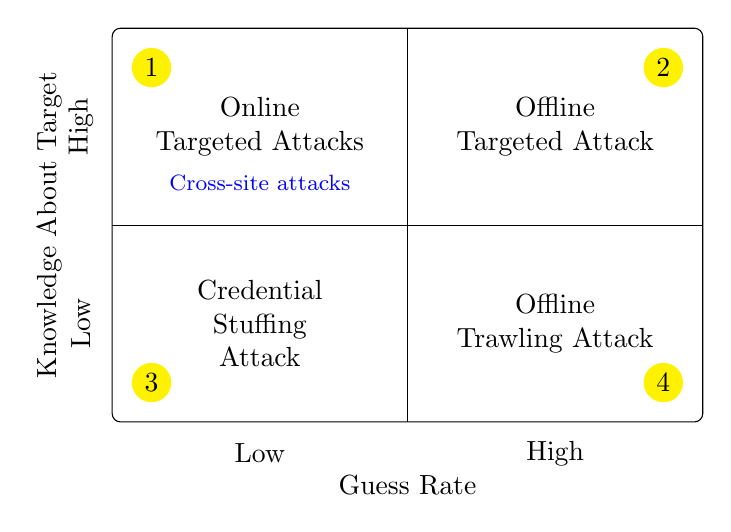
\begin{tikzpicture}
    % Variables for the grid size
    \def\gridwidth{7.5}
    \def\gridheight{5}

    % Draw the main grid
    \draw[rounded corners=3pt] (0,0) rectangle (\gridwidth,\gridheight);
    
    % Draw the dividing lines
    \draw (\gridwidth/2,0) -- (\gridwidth/2,\gridheight);
    \draw (0,\gridheight/2) -- (\gridwidth,\gridheight/2);
    
    % Labels for the attack types
    \node[align=center] (box1) at (\gridwidth/4,3*\gridheight/4) {Online\\Targeted Attacks};
    \node[align=center] at (3*\gridwidth/4,3*\gridheight/4) {Offline\\Targeted Attack};
    \node[align=center] at (\gridwidth/4,\gridheight/4) {Credential\\Stuffing\\Attack};
    \node[align=center] at (3*\gridwidth/4,\gridheight/4) {Offline\\Trawling Attack};

    \node[below, text=blue, font=\footnotesize] at (box1.south) {Cross-site attacks};
    
    % Labels for the axes
    \node[align=center] at (\gridwidth/2,-0.8) {Guess Rate};
    \node[align=center, rotate=90] at (-0.8,\gridheight/2) {Knowledge About Target};
    
    % Axis numbers
    \node[align=center] at (\gridwidth/4,-0.4) {Low};
    \node[align=center] at (3*\gridwidth/4,-0.4) {High};
    \node[align=center, rotate=90] at (-0.4,3*\gridheight/4) {High};
    \node[align=center, rotate=90] at (-0.4,\gridheight/4) {Low};


    % Circles with numbers
    % Upper left
    \node[circle,fill=yellow,inner sep=0pt,minimum size=0.5cm] at (0.5,\gridheight-0.5) {1};
    % Upper right
    \node[circle,fill=yellow,inner sep=0pt,minimum size=0.5cm] at (\gridwidth-0.5,\gridheight-0.5) {2};
    % Lower left
    \node[circle,fill=yellow,inner sep=0pt,minimum size=0.5cm] at (0.5,0.5) {3};
    % Lower right
    \node[circle,fill=yellow,inner sep=0pt,minimum size=0.5cm] at (\gridwidth-0.5,0.5) {4};

\end{tikzpicture}
\caption{Categories of attacks based on the attack rate (available to the attacker) on the horizontal axis and the amount of knowledge the attacker has about the target on the vertical axis. High attack rate signifies that the attacker has access to the target's hash. A low attack rate means that the attacker is trying to attack a hash through a rate limited service.}
\label{fig:attack-types}
\end{figure}